\chapter{目的} \label{cha:introduction}

\section{光生成反応\ref{fig:test1}}

宇宙線ミューオンが核子(陽子、中性子)と起こす反応に光生成反応がある。
この反応は核子とミューオンから出てくる光子との反応である。
また、この反応によりできるハドロン中間状態は、核子(N)と光子($\gamma$)の不変質量が小さい場合は短寿命の共鳴状態に近い。
また、終状態にはハドロンの中でも最も質量の小さいパイオン($\pi$)と陽子(p)の2つの粒子が出てくると期待される。

\begin{figure}[H]
	\centering
	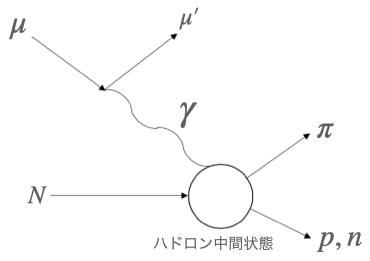
\includegraphics[width=10cm]{img/diagram_photoproduction.png}
	\caption{光生成反応のダイアグラム}
	\label{fig:test1}
\end{figure}